% Options for packages loaded elsewhere
\PassOptionsToPackage{unicode}{hyperref}
\PassOptionsToPackage{hyphens}{url}
\PassOptionsToPackage{dvipsnames,svgnames,x11names}{xcolor}
%
\documentclass[
  authoryear,
  preprint,
  3p]{elsarticle}

\usepackage{amsmath,amssymb}
\usepackage{lmodern}
\usepackage{iftex}
\ifPDFTeX
  \usepackage[T1]{fontenc}
  \usepackage[utf8]{inputenc}
  \usepackage{textcomp} % provide euro and other symbols
\else % if luatex or xetex
  \usepackage{unicode-math}
  \defaultfontfeatures{Scale=MatchLowercase}
  \defaultfontfeatures[\rmfamily]{Ligatures=TeX,Scale=1}
\fi
% Use upquote if available, for straight quotes in verbatim environments
\IfFileExists{upquote.sty}{\usepackage{upquote}}{}
\IfFileExists{microtype.sty}{% use microtype if available
  \usepackage[]{microtype}
  \UseMicrotypeSet[protrusion]{basicmath} % disable protrusion for tt fonts
}{}
\makeatletter
\@ifundefined{KOMAClassName}{% if non-KOMA class
  \IfFileExists{parskip.sty}{%
    \usepackage{parskip}
  }{% else
    \setlength{\parindent}{0pt}
    \setlength{\parskip}{6pt plus 2pt minus 1pt}}
}{% if KOMA class
  \KOMAoptions{parskip=half}}
\makeatother
\usepackage{xcolor}
\setlength{\emergencystretch}{3em} % prevent overfull lines
\setcounter{secnumdepth}{5}
% Make \paragraph and \subparagraph free-standing
\ifx\paragraph\undefined\else
  \let\oldparagraph\paragraph
  \renewcommand{\paragraph}[1]{\oldparagraph{#1}\mbox{}}
\fi
\ifx\subparagraph\undefined\else
  \let\oldsubparagraph\subparagraph
  \renewcommand{\subparagraph}[1]{\oldsubparagraph{#1}\mbox{}}
\fi


\providecommand{\tightlist}{%
  \setlength{\itemsep}{0pt}\setlength{\parskip}{0pt}}\usepackage{longtable,booktabs,array}
\usepackage{calc} % for calculating minipage widths
% Correct order of tables after \paragraph or \subparagraph
\usepackage{etoolbox}
\makeatletter
\patchcmd\longtable{\par}{\if@noskipsec\mbox{}\fi\par}{}{}
\makeatother
% Allow footnotes in longtable head/foot
\IfFileExists{footnotehyper.sty}{\usepackage{footnotehyper}}{\usepackage{footnote}}
\makesavenoteenv{longtable}
\usepackage{graphicx}
\makeatletter
\def\maxwidth{\ifdim\Gin@nat@width>\linewidth\linewidth\else\Gin@nat@width\fi}
\def\maxheight{\ifdim\Gin@nat@height>\textheight\textheight\else\Gin@nat@height\fi}
\makeatother
% Scale images if necessary, so that they will not overflow the page
% margins by default, and it is still possible to overwrite the defaults
% using explicit options in \includegraphics[width, height, ...]{}
\setkeys{Gin}{width=\maxwidth,height=\maxheight,keepaspectratio}
% Set default figure placement to htbp
\makeatletter
\def\fps@figure{htbp}
\makeatother

\makeatletter
\makeatother
\makeatletter
\makeatother
\makeatletter
\@ifpackageloaded{caption}{}{\usepackage{caption}}
\AtBeginDocument{%
\ifdefined\contentsname
  \renewcommand*\contentsname{Table of contents}
\else
  \newcommand\contentsname{Table of contents}
\fi
\ifdefined\listfigurename
  \renewcommand*\listfigurename{List of Figures}
\else
  \newcommand\listfigurename{List of Figures}
\fi
\ifdefined\listtablename
  \renewcommand*\listtablename{List of Tables}
\else
  \newcommand\listtablename{List of Tables}
\fi
\ifdefined\figurename
  \renewcommand*\figurename{Figure}
\else
  \newcommand\figurename{Figure}
\fi
\ifdefined\tablename
  \renewcommand*\tablename{Table}
\else
  \newcommand\tablename{Table}
\fi
}
\@ifpackageloaded{float}{}{\usepackage{float}}
\floatstyle{ruled}
\@ifundefined{c@chapter}{\newfloat{codelisting}{h}{lop}}{\newfloat{codelisting}{h}{lop}[chapter]}
\floatname{codelisting}{Listing}
\newcommand*\listoflistings{\listof{codelisting}{List of Listings}}
\makeatother
\makeatletter
\@ifpackageloaded{caption}{}{\usepackage{caption}}
\@ifpackageloaded{subcaption}{}{\usepackage{subcaption}}
\makeatother
\makeatletter
\@ifpackageloaded{tcolorbox}{}{\usepackage[many]{tcolorbox}}
\makeatother
\makeatletter
\@ifundefined{shadecolor}{\definecolor{shadecolor}{rgb}{.97, .97, .97}}
\makeatother
\makeatletter
\makeatother
\journal{Journal of Behavioral and Experimental Economics}
\ifLuaTeX
  \usepackage{selnolig}  % disable illegal ligatures
\fi
\usepackage[]{natbib}
\bibliographystyle{elsarticle-harv}
\IfFileExists{bookmark.sty}{\usepackage{bookmark}}{\usepackage{hyperref}}
\IfFileExists{xurl.sty}{\usepackage{xurl}}{} % add URL line breaks if available
\urlstyle{same} % disable monospaced font for URLs
\hypersetup{
  pdftitle={Growth and inequality in public good provision \textbar{} an extended replication},
  pdfauthor={Hauke Roggenkamp},
  pdfkeywords={Replication study, Non-convenience sample, Open
science, Dynamic public good game, Online experiment, Generalizability},
  colorlinks=true,
  linkcolor={blue},
  filecolor={Maroon},
  citecolor={Blue},
  urlcolor={Blue},
  pdfcreator={LaTeX via pandoc}}

\setlength{\parindent}{6pt}
\begin{document}

\begin{frontmatter}
\title{Growth and inequality in public good provision \textbar{} an
extended replication}
\author[1,2]{Hauke Roggenkamp%
%
}
 \ead{hauke.roggenkamp@unisg.ch} 

\affiliation[1]{organization={Helmut Schmidt
University},addressline={Holstenhofweg
85},city={Hamburg},postcode={22043}}
\affiliation[2]{organization={University of
St.~Gallen},addressline={Torstrasse
25},city={St.~Gallen},postcode={9000}}

\cortext[cor1]{Corresponding author}

        
\begin{abstract}
This is the abstract. Lorem ipsum dolor sit amet, consectetur adipiscing
elit. Vestibulum augue turpis, dictum non malesuada a, volutpat eget
velit. Nam placerat turpis purus, eu tristique ex tincidunt et. Mauris
sed augue eget turpis ultrices tincidunt. Sed et mi in leo porta
egestas. Aliquam non laoreet velit. Nunc quis ex vitae eros aliquet
auctor nec ac libero. Duis laoreet sapien eu mi luctus, in bibendum leo
molestie. Sed hendrerit diam diam, ac dapibus nisl volutpat vitae.
Aliquam bibendum varius libero, eu efficitur justo rutrum at. Sed at
tempus elit.
\end{abstract}





\begin{keyword}
    Replication study \sep Non-convenience sample \sep Open
science \sep Dynamic public good game \sep Online experiment \sep 
    Generalizability
\end{keyword}
\end{frontmatter}\ifdefined\Shaded\renewenvironment{Shaded}{\begin{tcolorbox}[breakable, boxrule=0pt, borderline west={3pt}{0pt}{shadecolor}, frame hidden, interior hidden, sharp corners, enhanced]}{\end{tcolorbox}}\fi

\begin{center}\rule{0.5\linewidth}{0.5pt}\end{center}

\textbf{Hintergrund:} Ich habe diesen
\href{https://groups.google.com/g/esa-announce/c/-_2OmbkdxEk}{post}
gesehen und überlege meine Replikation entsprechend
\href{https://www.sciencedirect.com/journal/journal-of-behavioral-and-experimental-economics/about/call-for-papers\#transparency-reproducibility-and-generalizability-of-behavioral-economics-experiments}{hier}
einzureichen. Ist das realistisch? Wenn ja, wie soll man die Story
aufziehen? Soll man denen mal schreiben und fragen, ob noch Platz ist?

\begin{center}\rule{0.5\linewidth}{0.5pt}\end{center}

\begin{quote}
``There are two possible articles you can write: (a) the article you
planned to write when you designed your study or (b) the article that
makes the most sense now that you have seen the results. They are rarely
the same, and the correct answer is (b).'' \citep[p.~171]{bemwriting}
\end{quote}

\hypertarget{pre-registered-gmtv-replication}{%
\section{Pre-registered GMTV
Replication}\label{pre-registered-gmtv-replication}}

\hypertarget{provision-of-the-public-good}{%
\subsection{Provision of the public
good}\label{provision-of-the-public-good}}

First, we ask whether the samples differ with respect to their initial
contributions to the public good. Is our replication sample more
pro-social than the original sample? Figure 1 reveals, that it is not.
The distributions of both samples look fairly similar. Both samples
contributed 10 tokens, that is, 50\% of their endowments on average
(median and mean).\footnote{The two-sided rank sum test (comparing
  differences between samples) yields a p-Value of 0.3926 for the mean
  contribution in first round of the game.} Moreover, both samples'
initial contributions resemble initial contributions participants
usually make in the standard game with partner matching.\footnote{See
  Figure 3B in \citet{fehrgaechter2000} (p.989), for instance.} In the
dynamic game presented here, we are particularly interested in the
subsequent periods because differences add up exponentially. Do the two
groups remain similar?

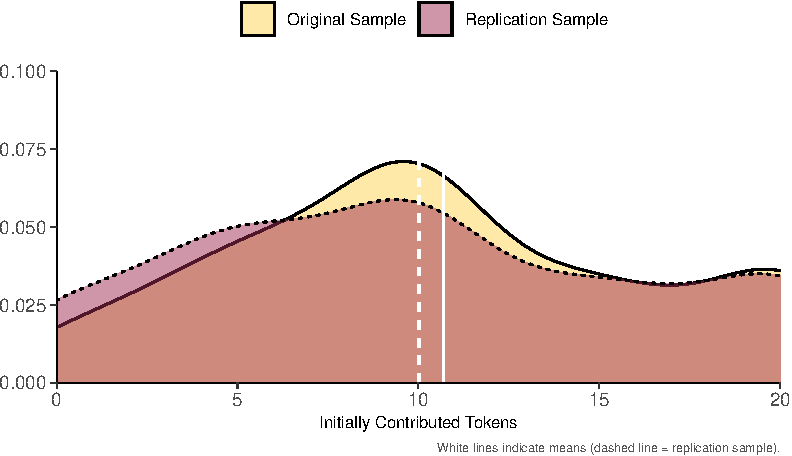
\includegraphics{paper_files/figure-pdf/firstRoundViz-1.pdf}

In particular, do the two samples' contributions follow the same pattern
over time? The answer is \emph{no}. Figure 2 illustrates that the
samples make similar contributions at the beginning and the end of the
game but behave differently in between. More precisely, the left
panel--depicting the average contributions in absolute terms--shows that
the original sample contributed substantially more than the replication
sample \emph{in all but the first and last rounds}. For this reason, the
original sample's behavior differs from the replication sample's
behavior in two aspects: it contributes more and exhibits a considerable
drop in the last period (whereas the replication sample's contributions
flatten). Note that increasing contributions over time imply increasing
endowments over time. Hence, increasing absolute contributions do not
necessarily imply that participants contribute increasing shares of
their endowments. The right panel in Figure 1 shows the share of overall
endowments contributed over time where both samples exhibit a similar
pattern: they decline and do not stabilize. The original sample's
behavior differs from the replication sample's behavior in one aspect:
it declined slower (to the same level in the last period).

\begin{figure}

{\centering 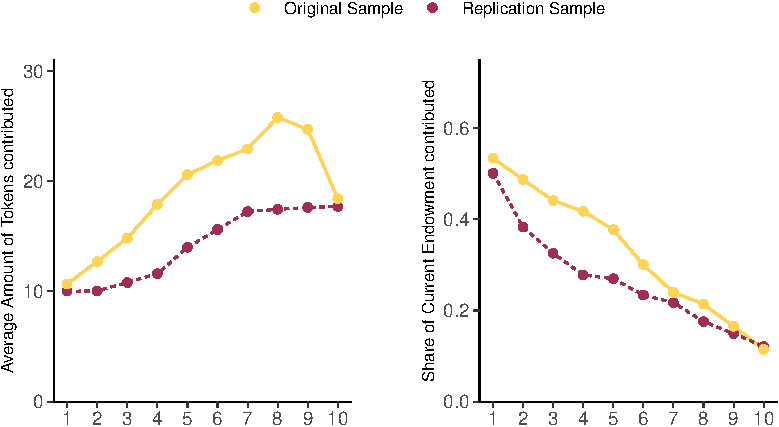
\includegraphics{paper_files/figure-pdf/plotShareOfContributions-1.pdf}

}

\caption{The average amount of tokens contributed over time in
treatments.}

\end{figure}

Moreover, both samples' contributions resemble contributions
participants usually make in the standard game with partner
matching.\footnote{The right panel is thus, comparable to the
  visualizations \emph{and results} in the standard game. See, for
  instance, Figure 1B in \citet{fehrgaechter2000} (p.986).} In the
dynamic game presented here, different paths lead to different levels of
wealth -- even if they share the same start- and end-points. We are
thus, more interested in the implications contributions have for wealth
generation and growth. So, how do the samples compare with respect to
wealth/income/endowments/stock?

\hypertarget{wealth-creation}{%
\subsection{Wealth Creation}\label{wealth-creation}}

How do the different contribution-paths translate to wealth?\footnote{To
  measure growth, we define a variable called \emph{stock} which sums
  the endowments of all participants in a given group at the end of the
  round (that is, after the contributions have been made, multiplied and
  redistributed).} Given that the original sample contributed more in
most of the periods, one would expect the respective groups to be
considerably more wealthy. Figure 3 indicates that they tend to be
insignificantly\footnote{The two-sided rank sum test (comparing
  differences between samples) yields a p-Value of 0.1356 for the mean
  stock in last round of the game.} richer.

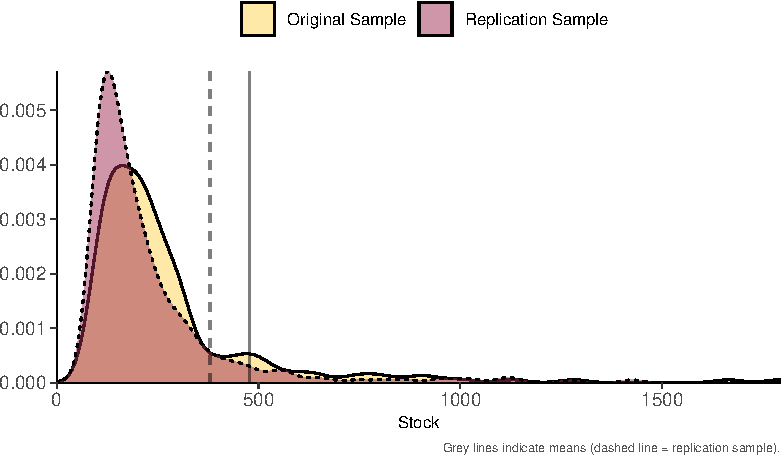
\includegraphics{paper_files/figure-pdf/stockDistributionViz-1.pdf}

As the grey lines indicate, an average group in the original sample
accumulated about 478 tokens. In contrast, an average group in the
replication sample accumulated about 380 tokens. However, none of the
groups were efficient: the maximal wealth that can be reached in round
10 under full cooperation is approximately 4613 tokens or 230 Euro per
group.

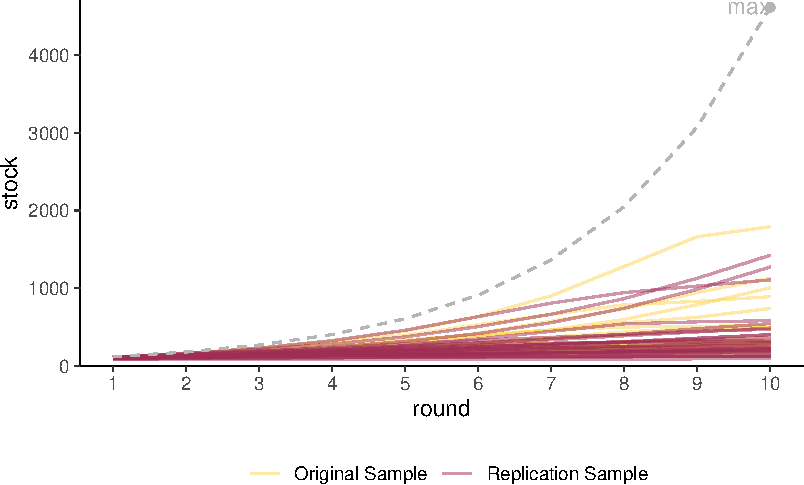
\includegraphics{paper_files/figure-pdf/growthHeterogeneityViz-1.pdf}

While there is clearly growth, groups do not realize the potential
efficiency as the replication groups reach on average a level of 379
tokens out of 4613 maximally possible or 8.2\%. As in the original data,
there is large heterogeneity with the richest group reaching 1425 tokens
whereas the poorest group ends up with 92 tokens.

We thus, observe growth even for the poorest group and spot
heterogeneity even within data sources.

Figure 2 shows the dynamics of wealth over time.\footnote{Unlike GMTV I
  present no median split but only the main results.}

\begin{figure}

{\centering 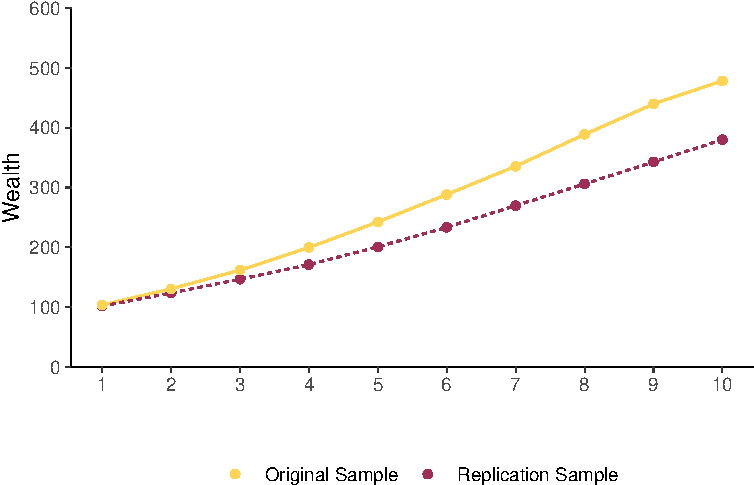
\includegraphics{paper_files/figure-pdf/plotStock-1.pdf}

}

\caption{Average wealth over time across treatments.}

\end{figure}

The Figure illustrates that (in both data sources) growth was continuous
and surprisingly linear, given the exponential character of the game's
design.

To sum up, our groups also tend to be poorer, and median wealth is
higher in GMTV. The difference in mean ranks is not significant
according to a two-sided ranksum test\footnote{The two-sided rank sum
  test (comparing differences between data sources) yields a p-Value of
  0.1356 for the mean wealth after the last round of the game.},
however.

To further assess the statistical significance of differences in means,
we run OLS regressions where we regress wealth on a treatment dummy for
\emph{Replication} (Table 3). These regressions show that differences in
means are only significant for below median groups. This implies that
the poor groups in our data are even less wealthy than GMTV's poor
groups.

\begin{table}[!htbp] \centering 
  \caption{} 
  \label{} 
\begin{tabular}{@{\extracolsep{5pt}}lccc} 
\\[-1.8ex]\hline 
\hline \\[-1.8ex] 
 & \multicolumn{3}{c}{\textit{Dependent variable:}} \\ 
\cline{2-4} 
\\[-1.8ex] & \multicolumn{3}{c}{Wealth} \\ 
 & All & Below median & Above median \\ 
\hline \\[-1.8ex] 
 Replication & $-$98.26 & $-$59.41$^{***}$ & $-$138.21 \\ 
  & (101.21) & (18.32) & (166.67) \\ 
  & & & \\ 
 Constant & 478.09$^{***}$ & 234.70$^{***}$ & 731.00$^{***}$ \\ 
  & (75.58) & (13.99) & (124.73) \\ 
  & & & \\ 
\hline \\[-1.8ex] 
Observations & 52 & 24 & 25 \\ 
R$^{2}$ & 0.02 & 0.32 & 0.03 \\ 
Residual Std. Error & 362.49 & 44.24 & 413.67 \\ 
\hline 
\hline \\[-1.8ex] 
\textit{Note:}  & \multicolumn{3}{r}{$^{*}$p$<$0.1; $^{**}$p$<$0.05; $^{***}$p$<$0.01} \\ 
\end{tabular} 
\end{table}

As such, our results look familiar to GMTV's findings, where poor groups
grew ever so slightly, while only rich groups experienced growth (that
became exponential only after the 10th round).


  \bibliography{../biblio.bib}


\end{document}
